% Options for packages loaded elsewhere
\PassOptionsToPackage{unicode}{hyperref}
\PassOptionsToPackage{hyphens}{url}
%
\documentclass[
]{article}
\usepackage{lmodern}
\usepackage{amssymb,amsmath}
\usepackage{ifxetex,ifluatex}
\ifnum 0\ifxetex 1\fi\ifluatex 1\fi=0 % if pdftex
  \usepackage[T1]{fontenc}
  \usepackage[utf8]{inputenc}
  \usepackage{textcomp} % provide euro and other symbols
\else % if luatex or xetex
  \usepackage{unicode-math}
  \defaultfontfeatures{Scale=MatchLowercase}
  \defaultfontfeatures[\rmfamily]{Ligatures=TeX,Scale=1}
\fi
% Use upquote if available, for straight quotes in verbatim environments
\IfFileExists{upquote.sty}{\usepackage{upquote}}{}
\IfFileExists{microtype.sty}{% use microtype if available
  \usepackage[]{microtype}
  \UseMicrotypeSet[protrusion]{basicmath} % disable protrusion for tt fonts
}{}
\makeatletter
\@ifundefined{KOMAClassName}{% if non-KOMA class
  \IfFileExists{parskip.sty}{%
    \usepackage{parskip}
  }{% else
    \setlength{\parindent}{0pt}
    \setlength{\parskip}{6pt plus 2pt minus 1pt}}
}{% if KOMA class
  \KOMAoptions{parskip=half}}
\makeatother
\usepackage{xcolor}
\IfFileExists{xurl.sty}{\usepackage{xurl}}{} % add URL line breaks if available
\IfFileExists{bookmark.sty}{\usepackage{bookmark}}{\usepackage{hyperref}}
\hypersetup{
  hidelinks,
  pdfcreator={LaTeX via pandoc}}
\urlstyle{same} % disable monospaced font for URLs
\usepackage{graphicx}
\makeatletter
\def\maxwidth{\ifdim\Gin@nat@width>\linewidth\linewidth\else\Gin@nat@width\fi}
\def\maxheight{\ifdim\Gin@nat@height>\textheight\textheight\else\Gin@nat@height\fi}

\makeatother
% Scale images if necessary, so that they will not overflow the page
% margins by default, and it is still possible to overwrite the defaults
% using explicit options in \includegraphics[width, height, ...]{}
\setkeys{Gin}{width=\maxwidth,height=\maxheight,keepaspectratio}
% Set default figure placement to htbp
\makeatletter
\def\fps@figure{htbp}
\makeatother
\setlength{\emergencystretch}{3em} % prevent overfull lines
\providecommand{\tightlist}{%
  \setlength{\itemsep}{0pt}\setlength{\parskip}{0pt}}
\setcounter{secnumdepth}{-\maxdimen} % remove section numbering

\author{}
\date{}
\setlength{\evensidemargin}{8mm} 
\setlength{\oddsidemargin}{8mm}
\setlength{\textwidth}{150mm}
\begin{document}
\hypertarget{header-n0}{%
\subsection{Psychological first-aid model in COVID-19 inpatients in Wuhan}\label{header-n0}}

\vspace{5mm}
\textbf{Wenhong Cheng, M.D.$^{1,2,*}$, Fang Zhang, M.Ed.$^1$, Yingqi Hua, M.D., Ph.D.$^3$, Zhi Yang Ph.D.$^{4,5}$, and Jun Liu, M.D., Ph.D.$^{6,**}$}
\vspace{5mm}

1 Department of Psychiatry, Shanghai General Hospital, Shanghai Jiao Tong University School of Medicine.

2 Department of Child and Adolescent Psychiatry, Shanghai Mental Health Center, Shanghai Jiao Tong University School of Medicine.

3 Department of Scientific Administration, Shanghai General Hospital, Shanghai Jiao Tong University School of Medicine.

4 Laboratory of Psychological Health and Imaging, Shanghai Mental Health Center, Shanghai Jiao Tong University School of Medicine. 

5 Institute of Psychological and Behavioral Science, Shanghai Jiao Tong University.

6 Department of Nephrology, Shanghai General Hospital, Shanghai Jiao Tong University School of Medicine.

-- all in Shanghai, China

* Corresponding Author: Wenhong Cheng, chengwhb@aliyun.com

** Corresponding Author: Jun Liu, liujun-sgh@sjtu.edu.cn
\vspace{5mm}

\textbf{Abstract}

The sudden outbreak of COVID-19, as well as the substantial shortage of local health care resources, has led to panic experiences in many patients. Patients flooded to hospitals for diagnosis and treatment, waited in a long list for a hospital bed, witnessed sudden deaths, and suffered from the illness in Wuhan, the eye of the storm. While it is well recognized that psychological first-aid in this situation is essential, the lack of psychiatrists and the closed-ward environment have challenged the efforts to provide psychological first-aid.  
We are a medical team stationed in Leishenshan Hospital, Wuhan, China, starting from February this year. The team has a total of 156 staff members, and only one psychiatrist is with the team. Facing the unique difficulties, we have developed a psychological intervention system for patients in the hospital. The system has been functioning for more than a month and has demonstrated good effectiveness and efficiency. 
We think that medical teams around the world may be or are about to face the same problems as us. Therefore, it is an obligation for us to introduce the in-hospital psychological intervention system that we have designed and tested to our colleagues around the world.

\newpage

Due to the high contagiousness of COVID-19, more than 80,000 cases were confirmed in China, and up till now, over one million cases have been confirmed worldwide since the outbreak. In addition, the mortality of COVID-19 in Italy has reached close to 11\%, which is the highest in the world. The sudden outbreak of COVID-19, as well as the substantial shortage of local health care providers, personal protective equipment (PPE) and resuscitation devices, has led to panic experiences in many patients. Patients flooded to the hospital for diagnosis and treatment, waited in a long list for a hospital bed, witnessed sudden death, and suffered from the illness in Wuhan, the eye of the storm. A study in China found that in the past two months, inpatients with COVID-19 widely suffered from anxiety, depression, and other stress-related symptoms$^1$. Studies have shown that psychological reactions due to catastrophic events have adverse effects on physical recovery$^2$. Early psychological intervention can help rebuild trust and self-control feelings, reduce physical and mental symptoms, and prevent posttraumatic stress disorder (PTSD)$^3$. The WHO suggested that psychological first aid should be provided to those who were impacted when a disaster occurred, as well as in the days or weeks following the disaster, with particular focus on groups that need more attention, including those who lack social support and who are severely affected and in poor health condition$^4$. However, it is undoubtedly a challenge to provide psychological help for this group of patients in the setting of closed wards.

In our clinical practice, we found that after experiencing the negative social period caused by the COVID-19 outbreak in January 2020, many patients showed stress symptoms, such as increased vigilance, depression, anxiety, irritability, flashbacks and or nightmares, feelings of being discriminated or rejected, and loneliness caused by the infectious disease. These symptoms would aggravate the patients' chest distress, palpitations, and other physical symptoms. In the medical environment, patients were afraid of closed wards. Most of the patients had family members who were also diagnosed with COVID-19 at different quarantine locations, and some of them lost their family members who died from COVID-19. As a result of quarantine, no family members or friends could visit them. They felt strange when facing doctors from other provinces with non-native dialects. Most critically, there was a lack of on-site psychological workers; medical care providers well-gowned with PPE in the closed ward of infectious diseases cannot stay for a long time, and it is inconvenient to talk to patients wearing protective clothing. All the above factors bring limitations to the traditional psychological face-to-face diagnosis. We developed an integrated on-site & online psychological intervention program for this particular situation, where only one psychotherapist (psychiatrist) provided psychological assistance to a total of 90 patients in two wards at Leishenshan Hospital in Wuhan, the newly-built infectious disease hospitals. The primary goal of the program was to reduce patients' psychosomatic symptoms, promote recovery, enhance feelings of safety and resilience, and prevent PTSD. The main intervention principles were to provide health education, stabilize fearful emotions, increase social-supportive links, promote problem-solving, and encourage or inspire patients using their resources (see Figure 1).

First, we provide reading materials, discussion, and lectures online to help doctors and nurses identify depression and acute stress reaction or disease symptoms and learn simple intervention and referral skills. A psychiatrist would go into the ward and briefly communicate with each patient so they could get to know each other. Then, we invited patients to join an online patient-support group through WeChat, a wildly used social media app. In an online daily one-hour support group meeting, psychiatrists facilitated discussion. They provided counseling for disease information, rehabilitation training, emotion regulation, and sleep education, and she could also identify individuals who needed further individual online consultation. We found that at the beginning, a high frequency of individual psycho-counseling at least three sessions per week were usually required. We found that it is essential to establish the initial trust in the relationship in the first brief contact with the patient in the ward. For more accessible communication in a closed ward, the psychiatrist wrote her name and department on the protective gown to let the patients know her quickly by reading the texts besides oral self-introduction. She asked brief semi-open questions such as, "Did you sleep well? How is your appetite?" The psychiatrist could perform the initial evaluation and sort patients with different mental conditions. Weekly follow-up rounds are also necessary to maintain online counseling depth. For patients who had lost a family member(s), depressive patients who had negative thoughts or passive thoughts, or patients who tended to meltdown due to severe anxiety, an offline session could often lead to a significant improvement. We found that offline communication, even a few times, had a synergistic therapeutic effect. It increased trust and reduced fear of abandonment, providing a basis for online intervention. To avoid burnout, we included an online counseling team consisting of psychotherapists, where psychiatrists played a role in making the treatment plan, performing referrals, and supervising.

\begin{figure}
\centering
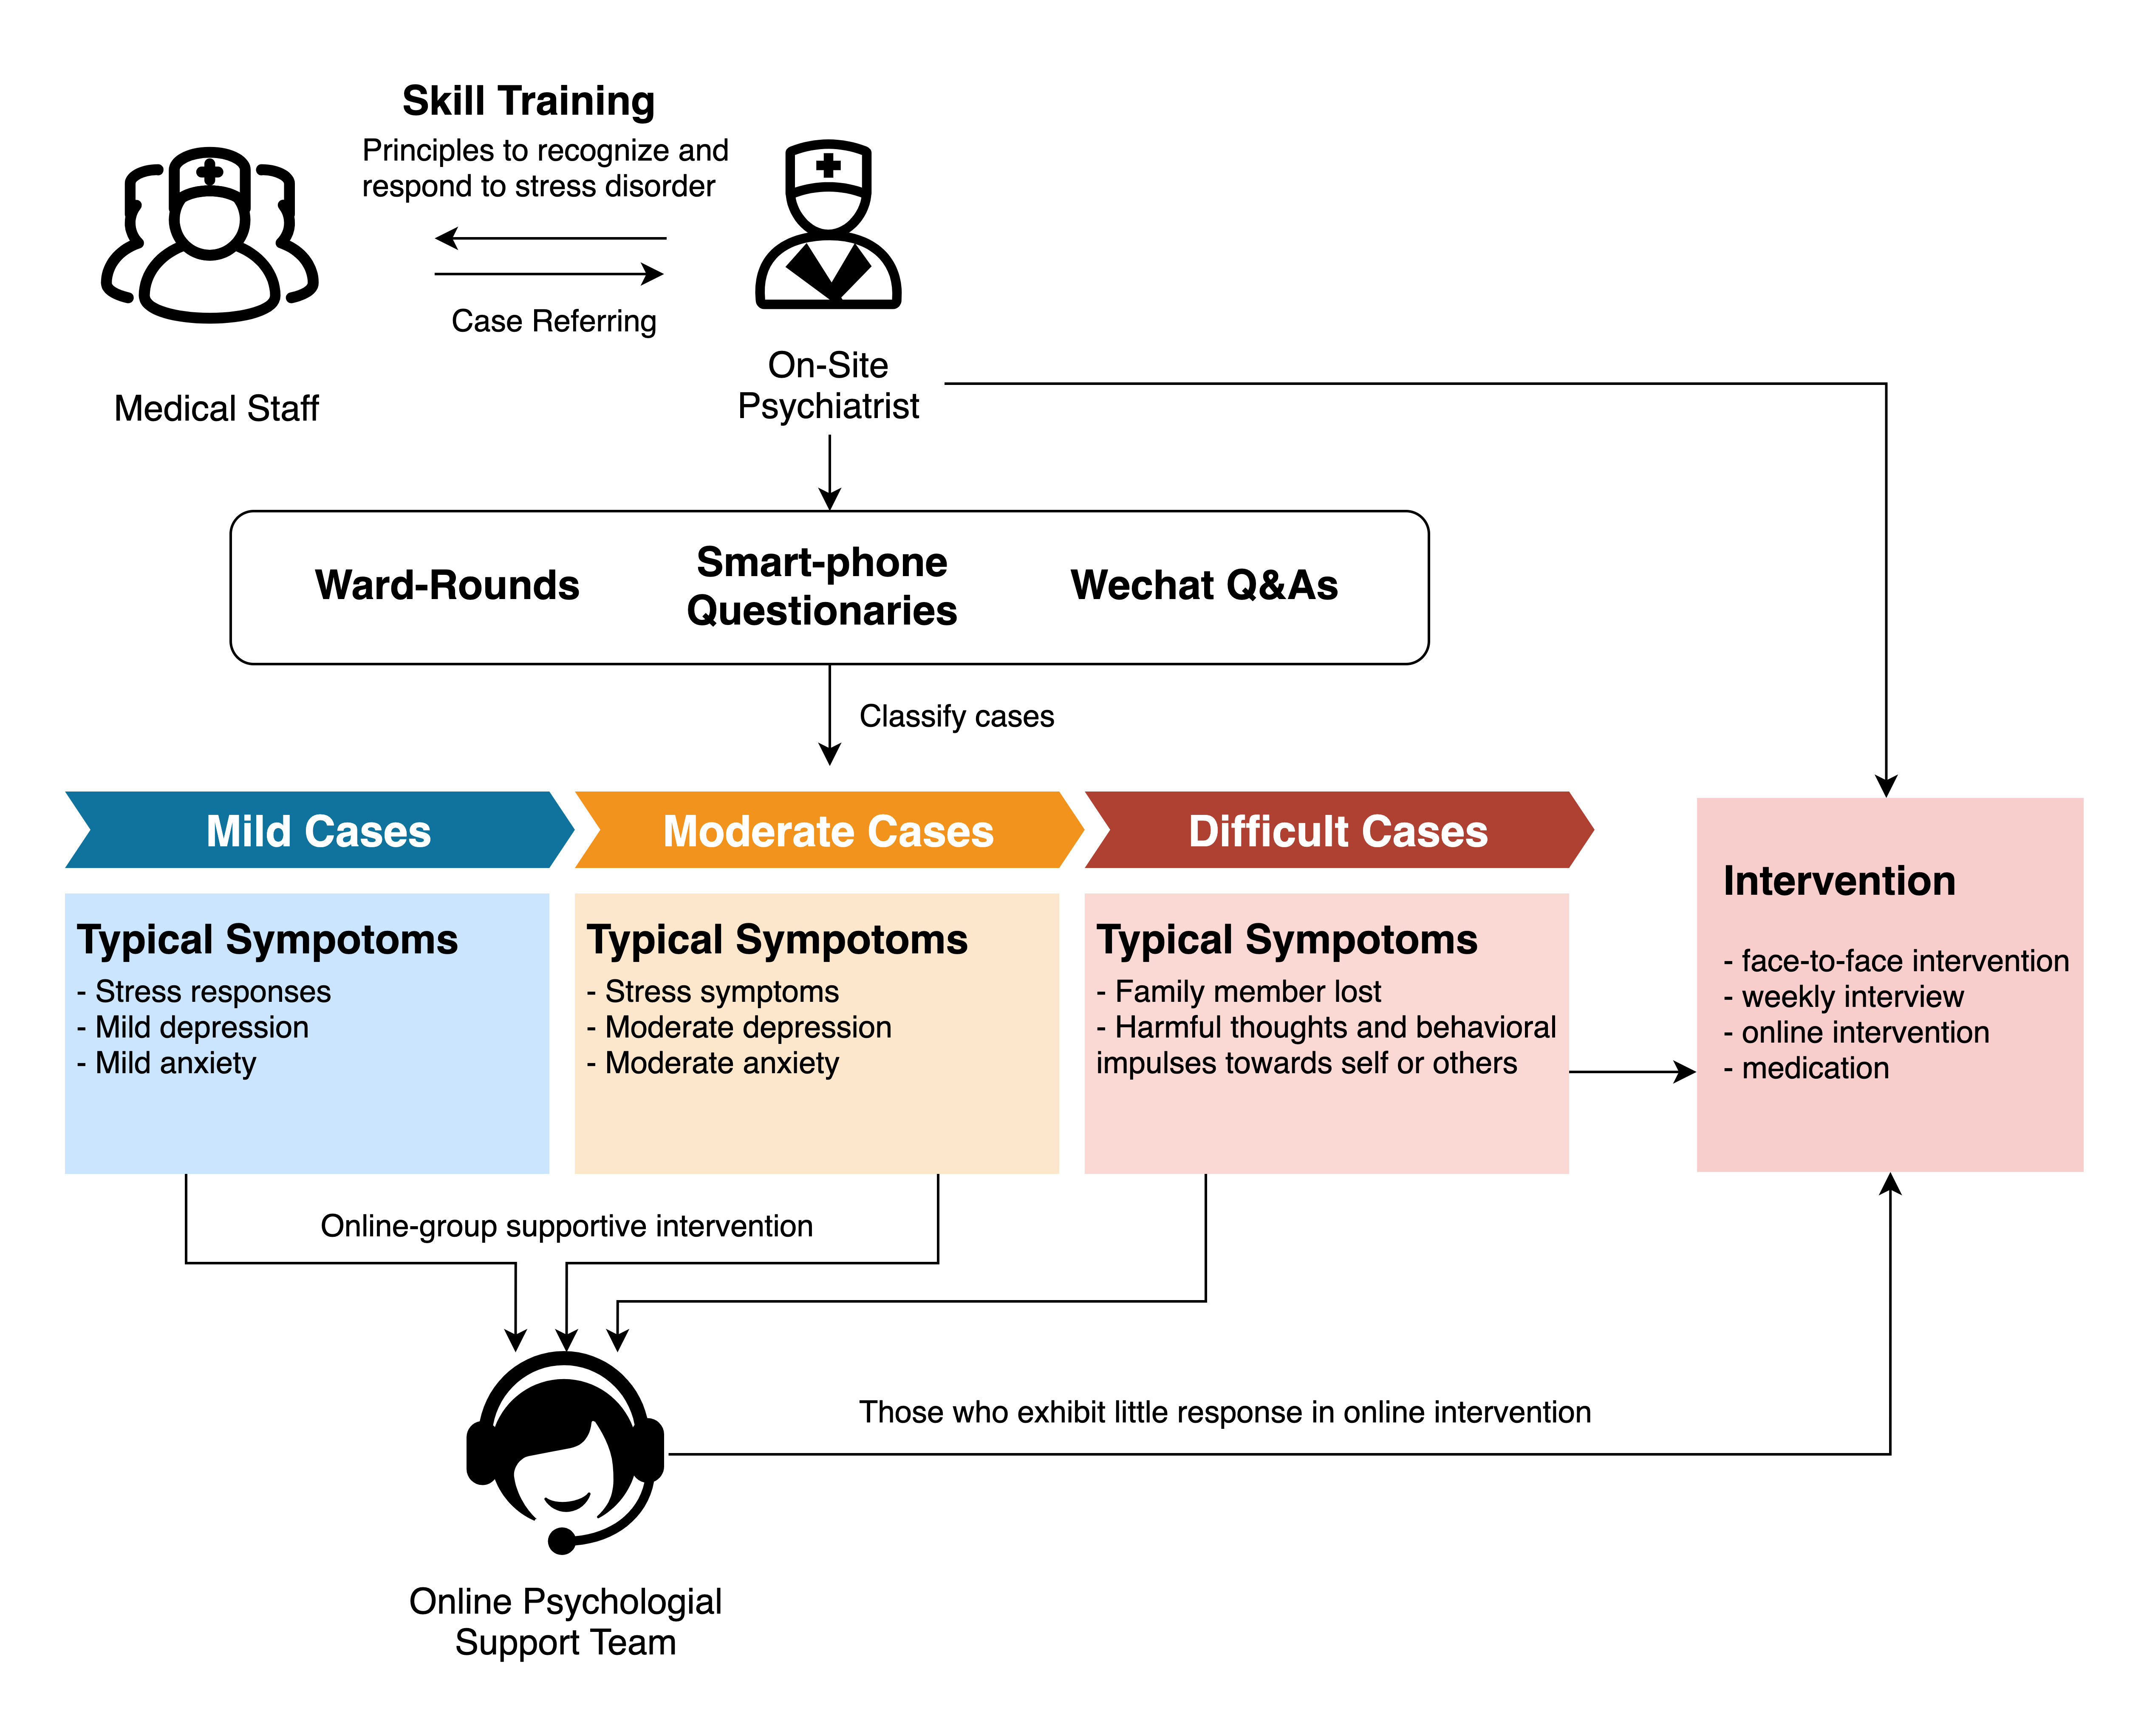
\includegraphics{fig_patient_workflow.jpg}
\caption{Psychological intervention model}
\end{figure}

We found that this model was useful to help patients. Many patients commented as: "Not only was my body treated but also the heart"; "In my most difficult time, I was pulled up by a psychiatrist; thus, I did not fall due to the disease and fear"; and "When I first came here, I felt very nervous, feeling increased chest distress and palpitations." It was psychological counseling that helped me in time to adjust my emotions. It was the first time for me to feel the spirit is the primary weapon to recover in the background of the disaster". In one case, the patient lost his father in the outbreak, and his infected mother was also in quarantine, was unaware of her husband's death. The patients had moderate depressive symptoms according to the questionnaire, but he was very passive to express them during the first contact and following online counseling. However, continuous online contact built trust between him and the psychiatrist. In the second week of offline consultation, the patient burst into tears and talked about his sorrow and worry. After that, his online interactions became active, and his symptoms improved. Our practice shows that, in the case of insufficient professional staff on the spot, the program we created was suitable for the psychological assistance of healthy socially isolated patients in a sudden outbreak of a highly infectious disease. It is challenging to obtain trust relying on solitary online psychological aid, and the compliance and effect are limited. Other teams in Leishenshan Hospital in Wuhan have applied this model in their daily practice.

Many countries have reached a consensus on the goal and significance of psychological assistance for large-scale disasters$^5$, and the implementation needs to be more flexible according to the characteristics of disasters and accessibility of medical resources. The outbreak of COVID-19 pandemic is a severe challenge to resources related to psychological services and routine diagnosis and treatment in various countries. We feel that this combination of on-site and online approaches can lead to more efficient psychological intervention, promote health, increase psychological adaptation, and prevent PTSD. This model could be adopted and adapted further all over the world.

\\
\textbf{References}

1. Zhao Q, Hu C, Feng R, et al. Investigation of the mental health of patients with novel coronavirus pneumonia. Chin J Neurol 2020;53.

2. Ryder AL, Azcarate PM, Cohen BE. PTSD and Physical Health. Curr Psychiatry Rep 2018;20(12):116.

3. Birur B, Moore NC, Davis LL. An evidence-based Review of Early Intervention and Prevention of Posttraumatic Stress Disorder. Community Ment Health J 2017;53:183-201.

4. World Health Organization. Psychological First Aid: Guide for field workers. WHO. 2011 (https://apps.who.int/iris/bitstream/handle/10665/44615/9786188273719-gre.pdf)

5. Inter-Agency Standing Committee Reference Group for Mental Health and Psychosocial Support in Emergency Settings. Briefing note on addressing mental health and psychosocial aspects of COVID-19 Outbreak. 2020;(Feb):1-20.


\end{document}


